\newpage
\section{Annexes}

\printglossaries
\printnomenclature
\begin{thebibliography}{9}
    \bibitem{soniccoloru}
    Sonic Team (3 septembre 2021) \emph{Sonic Colours Ultimate}, SEGA.
    
    \bibitem{learnopengl} 
    Joey de Vries, \textit{LearnOpenGL}.  
    Disponible en ligne : \url{https://learnopengl.com/}.  
    LearnOpenGL est une ressource en ligne exhaustive dédiée à l'apprentissage de la programmation graphique avec OpenGL.  
    Le site couvre des sujets tels que la manipulation des shaders, la gestion des textures, les transformations 3D,  
    ainsi que des concepts avancés comme le rendu différé et les ombres en temps réel.  
    Consulté le 1 avril 2025.

    \bibitem{imanolfotia} 
    Imanol Fotia, \textit{Blog - Article 1}.  
    Disponible en ligne : \url{https://imanolfotia.com/blog/1}.  
    Ce blog aborde divers sujets liés à la programmation, à l'ingénierie logicielle et aux technologies modernes.  
    Il propose des analyses approfondies, des tutoriels techniques et des réflexions sur les bonnes pratiques en développement.  
    Consulté le 1 avril 2025.

    \bibitem{iehl_deferred_vs_forward} 
    Jean-Claude Iehl, \textit{Deferred Shading vs Forward Shading}.  
    Disponible en ligne : \url{https://perso.univ-lyon1.fr/jean-claude.iehl/Public/educ/M2PROIMA/2018/deferred_vs_forward.html}.  
    Ce document pédagogique explique les différences entre le rendu différé (Deferred Shading) et le rendu direct (Forward Shading).  
    Il couvre les principes fondamentaux de chaque technique, leurs avantages et inconvénients, ainsi que leurs applications  
    dans les moteurs de rendu modernes.  
    Consulté le 1 avril 2025.

    \bibitem{courreges_doom2016} 
    Adrian Courrèges, \textit{DOOM (2016) - Graphics Study}.  
    Disponible en ligne : \url{https://www.adriancourreges.com/blog/2016/09/09/doom-2016-graphics-study/}.  
    Cet article propose une analyse approfondie du moteur graphique de *DOOM (2016)*, en explorant les techniques de rendu utilisées,  
    telles que le rendu différé, l'éclairage, la gestion des ombres, le post-traitement et l'optimisation des performances.  
    L'auteur décortique les effets visuels et les choix techniques ayant permis au jeu d'atteindre un haut niveau de fluidité et de qualité visuelle.  
    Consulté le 1 avril 2025.

    \bibitem{valve_source_engine} 
    Valve Corporation, \textit{Source Engine Features}.  
    Disponible en ligne : \url{https://developer.valvesoftware.com/wiki/Source_Engine_Features}.  
    Cette page du wiki officiel de Valve décrit les fonctionnalités du moteur Source, utilisé dans de nombreux jeux  
    comme *Half-Life 2*, *Portal* et *Counter-Strike: Source*. Elle couvre des aspects tels que le rendu graphique,  
    la gestion de la physique, le réseau, l'intelligence artificielle et les outils de développement fournis avec le moteur.  
    Consulté le 1 avril 2025.

    \bibitem{wikipedia_cryengine} 
    Wikipedia, \textit{CryEngine}.  
    Disponible en ligne : \url{https://en.wikipedia.org/wiki/CryEngine}.  
    Cet article de Wikipedia fournit une vue d'ensemble détaillée de CryEngine, un moteur de jeu développé par Crytek.  
    Il explore ses caractéristiques techniques, ses applications dans les jeux vidéo, ses versions successives et ses améliorations au fil du temps.  
    CryEngine est reconnu pour ses capacités de rendu photoréaliste et son utilisation dans des jeux populaires comme *Crysis*.  
    Consulté le 1 avril 2025.

    \bibitem{chanhaeng_normalparallax} 
    Chanhaeng, \textit{Normal/Parallax Mapping with Self-Shadowing}.  
    Disponible en ligne : \url{https://chanhaeng.blogspot.com/2019/01/normalparllax-mapping-with-self.html}.  
    Cet article explique en détail l'implémentation du normal mapping et du parallax mapping avec auto-ombrage.  
    L'auteur y décrit les concepts théoriques de ces techniques graphiques avancées et leur application dans les moteurs de rendu.  
    Le blog fournit également un code exemple pour implémenter ces effets dans les shaders.  
    Consulté le 1 avril 2025.

    \bibitem{silicon_graphics}
    Silicon Graphics.
    Disponible en ligne : \url{https://www.sgi.com/}.
    Silicon Graphics, Inc. (SGI) est une entreprise américaine spécialisée dans la conception de stations de travail et de superordinateurs.
    Pionnier dans le domaine de l'informatique graphique, elle est à l'origine de la création d'OpenGL,
    une API de rendu 2D et 3D largement adoptée dans l'industrie. Leur modèle de pipeline graphique a influencé
    de nombreux moteurs de jeu modernes, ayant fait ses preuves dans l'industrie du jeu vidéo lors de leur collaboration avec
    Nintendo en 1996 pour la création de la Nintendo 64 \cite{copetti_n64}.

    \bibitem{copetti_n64} 
    Fabio Copetti, \textit{Nintendo 64}.  
    Disponible en ligne : \url{https://www.copetti.org/writings/consoles/nintendo-64/}.  
    Cet article offre une analyse détaillée de la console Nintendo 64, y compris son architecture matérielle, ses composants, et les défis techniques rencontrés lors de son développement.  
    L'auteur explore également les innovations apportées par la N64, comme le processeur graphique et le stockage sur cartouche.  
    Consulté le 1 avril 2025.

    \bibitem{lalanguefrancaise}
    La Langue Française.
    Disponible en ligne : \url{https://www.lalanguefrancaise.com/}.
    La Langue Française est un site dédié à la langue française, proposant des ressources, des articles et des outils pour améliorer la maîtrise de la langue.
    Il aborde divers sujets tels que la grammaire, le vocabulaire, l'orthographe et la culture francophone.
    Le site est une référence pour les francophones souhaitant approfondir leur connaissance de la langue française.

    \bibitem{obj_format}
    Wavefront Technologies, \textit{OBJ File Format}.
    Disponible en ligne : \url{https://en.wikipedia.org/wiki/Wavefront_.obj_file}.
    Le format de fichier OBJ est un format de fichier standard pour représenter des objets 3D.
    Il est largement utilisé dans l'industrie de la modélisation 3D et est pris en charge par de nombreux logiciels de modélisation.
    Le format OBJ est simple et facile à lire, ce qui en fait un choix populaire pour l'échange de données 3D entre différentes applications.
    Il permet de stocker des informations sur la géométrie et éventuellement des textures, des matériaux et d'autres attributs associés à un objet 3D s'il est
    accompagné d'un fichier MTL.

    \bibitem{glsl}
    Khronos Group, \textit{OpenGL Shading Language (GLSL)}.
    Disponible en ligne : \url{https://www.khronos.org/opengl/wiki/OpenGL_Shading_Language}.
    OpenGL Shading Language (GLSL) est un langage de
    programmation de shaders de haut niveau dont la syntaxe est fondée sur
    le langage C.
    

\end{thebibliography}

\subsection{Exemples de débogage}

\begin{figure}[H]
    \begin{subfigure}{0.5\textwidth}
        \centering
        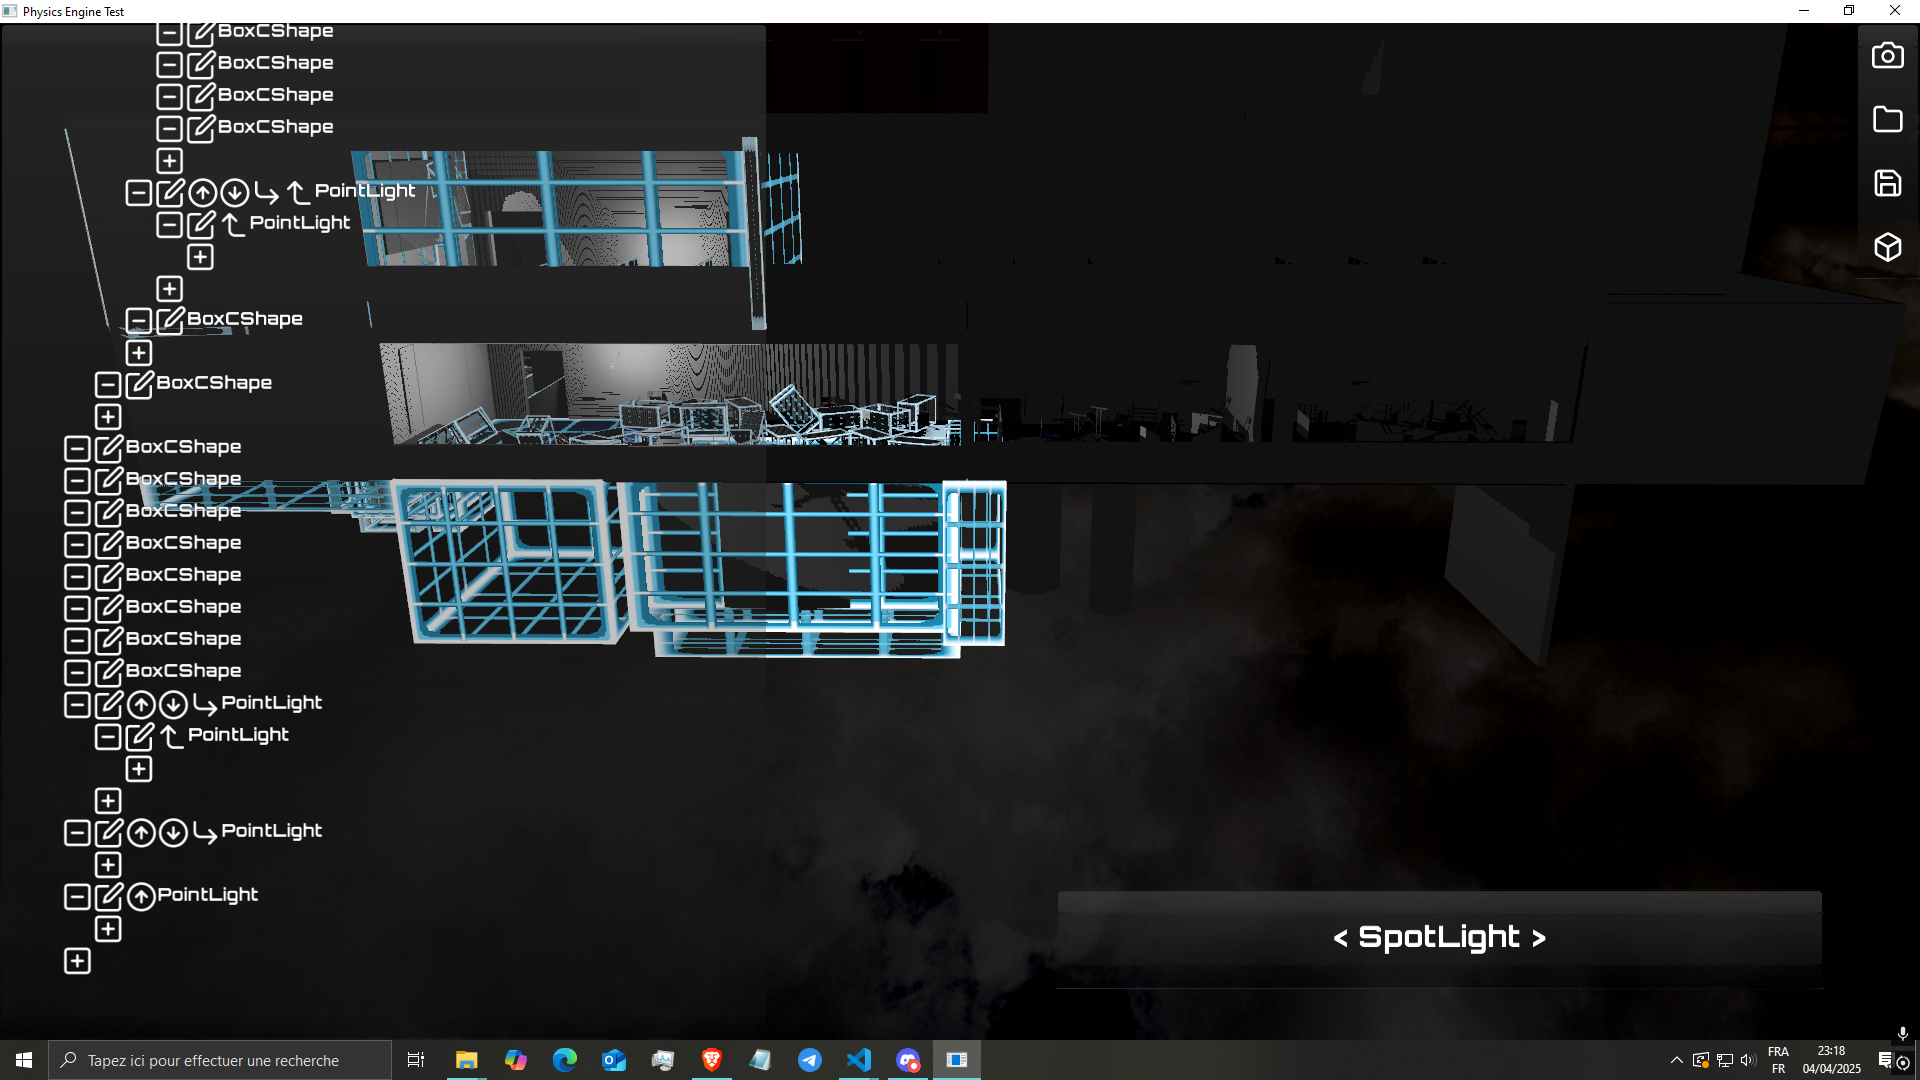
\includegraphics[width=0.8\textwidth]{images/gdb_editeur.png}
        \caption{Bug de collision}
        \label{fig:editeur1}
    \end{subfigure}
    \begin{subfigure}{0.5\textwidth}
        \centering
        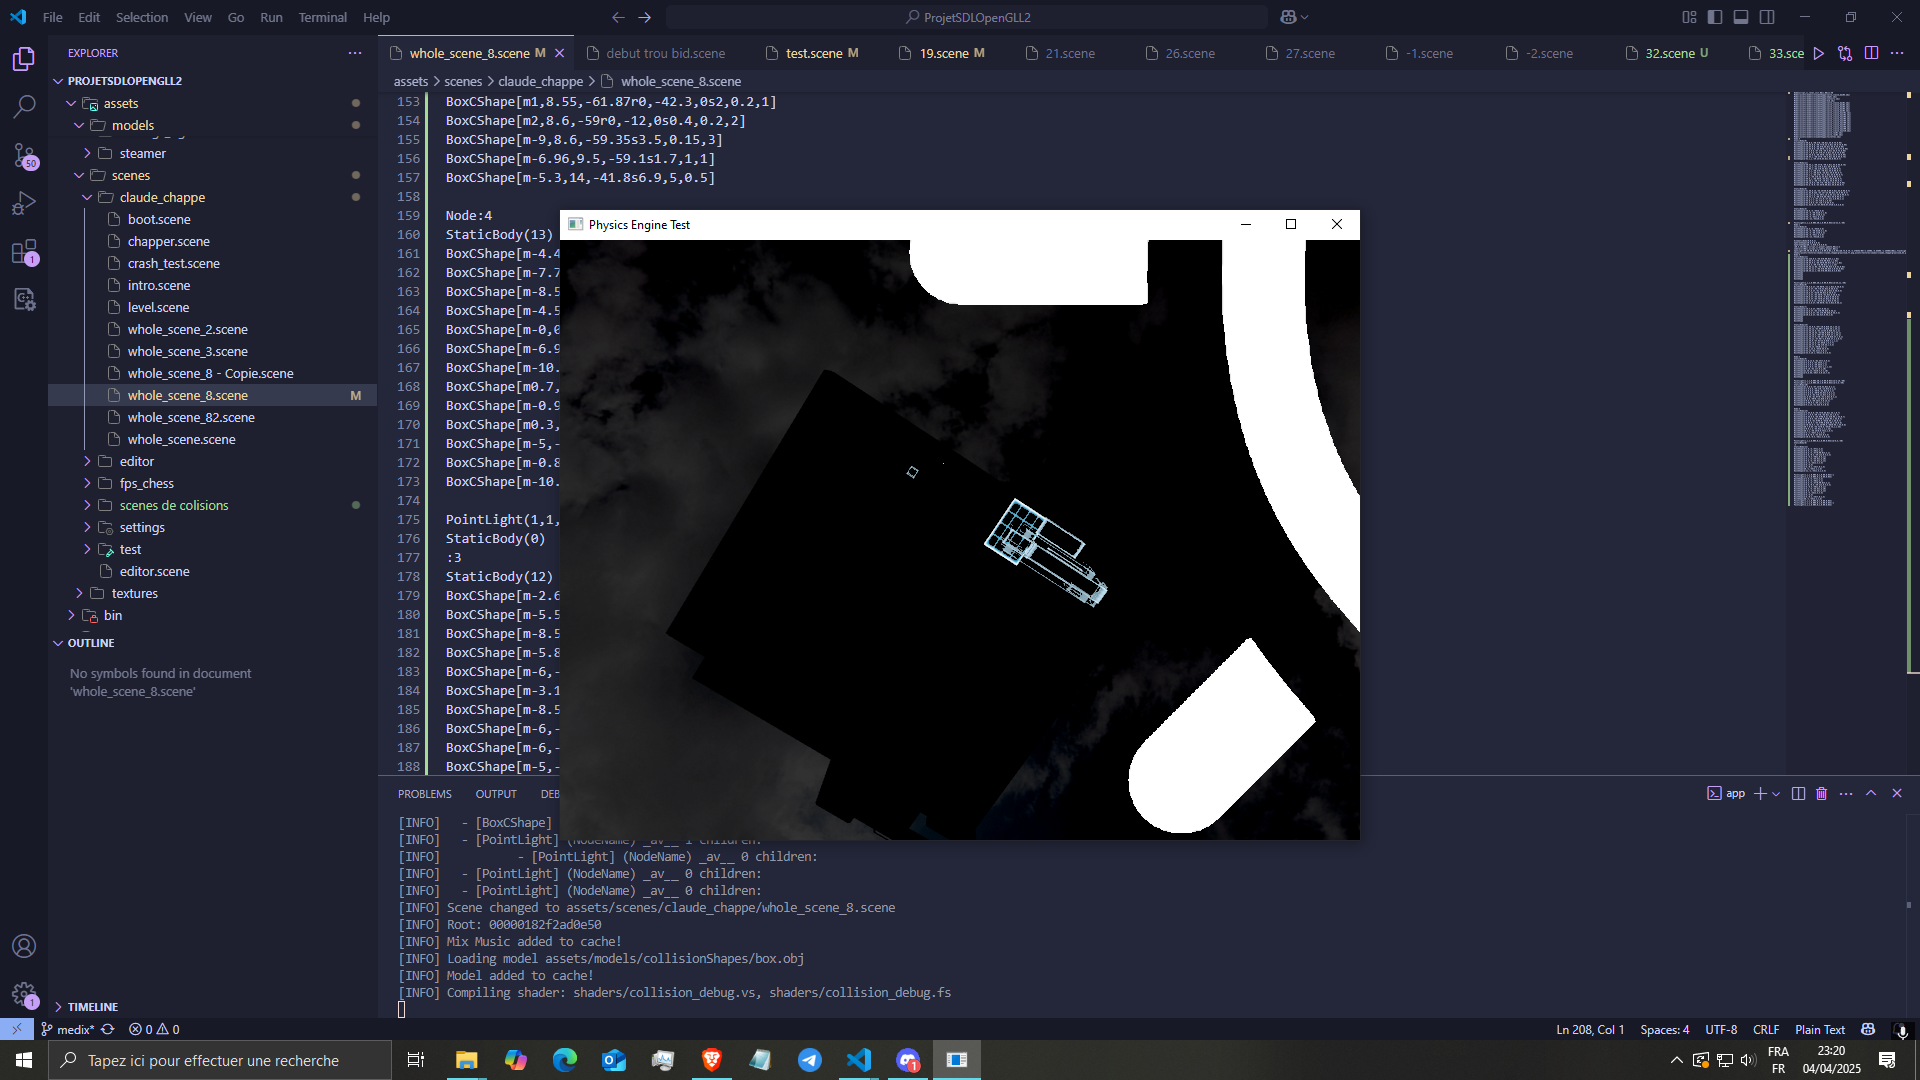
\includegraphics[width=0.8\textwidth]{images/gdb_editeur2.png}
        \caption{Bug de collision}
        \label{fig:editeur2}
    \end{subfigure}
    \begin{subfigure}{0.5\textwidth}
        \centering
        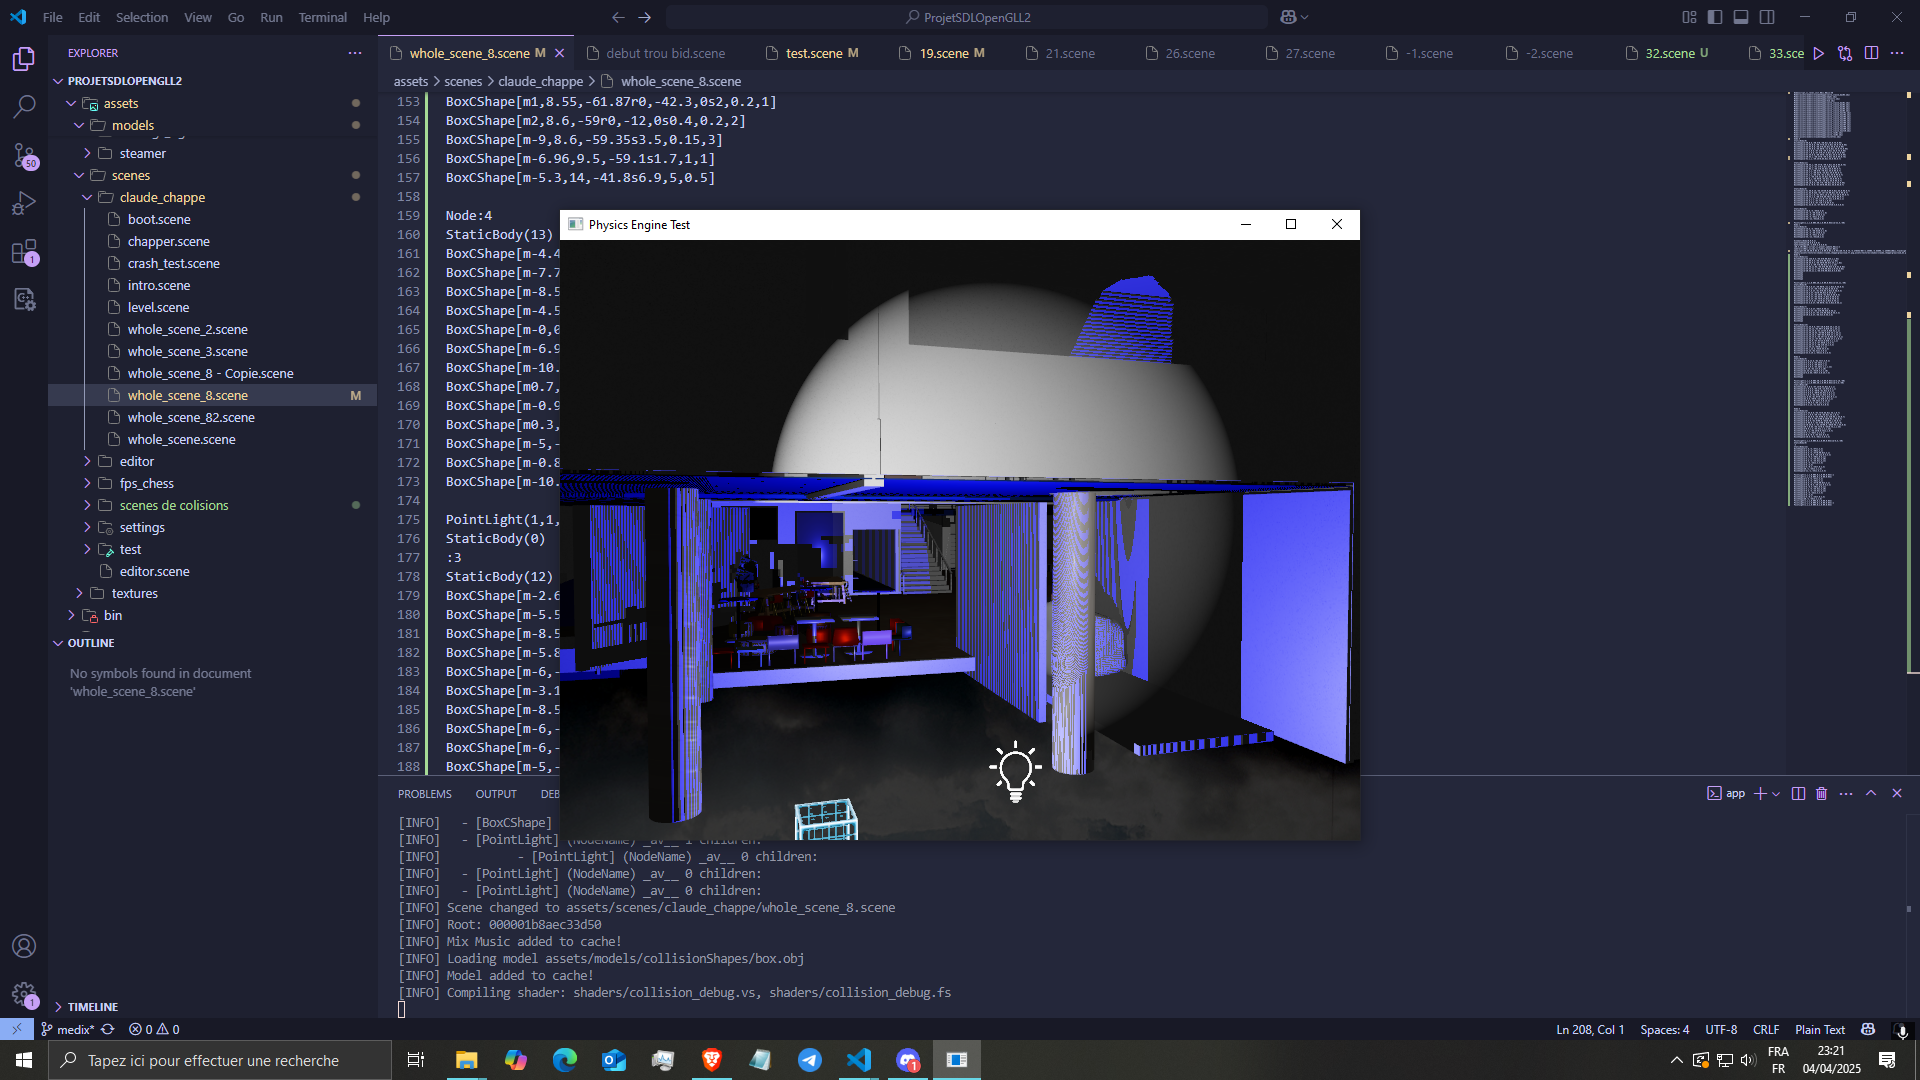
\includegraphics[width=0.8\textwidth]{images/gdb_editeur3.png}
        \caption{Bug d'affichage}
        \label{fig:editeur3}
    \end{subfigure}
    \caption{Exemples de bug à déboguer}
    \label{fig:debug}
\end{figure}

\begin{multicols}{2}
\begin{figure}[H]
    \centering
    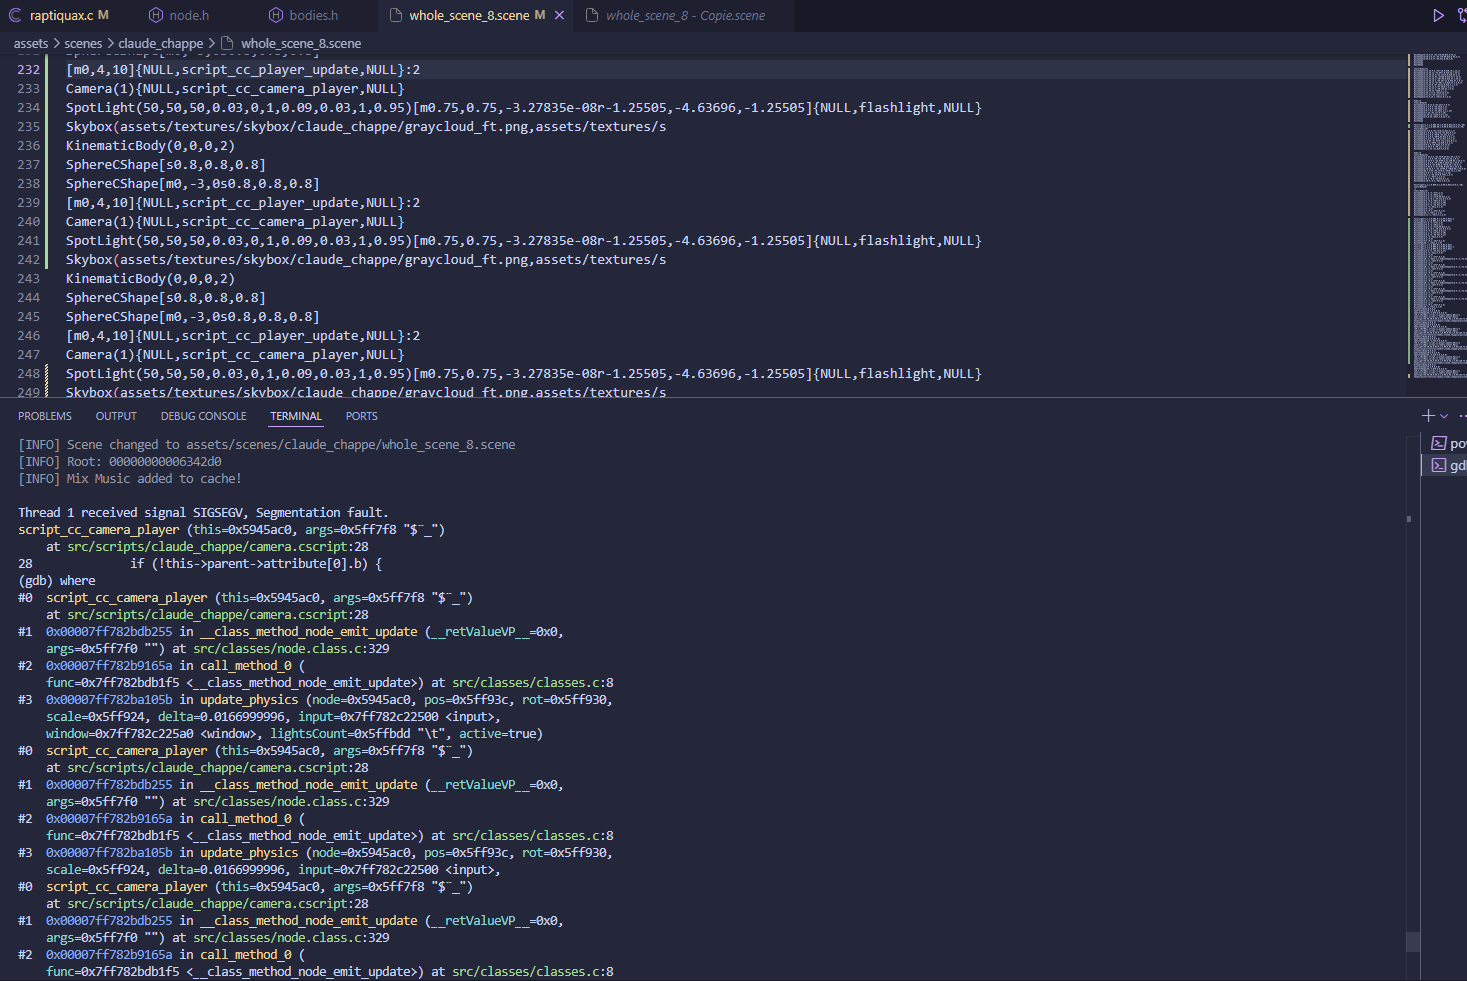
\includegraphics[width=0.5\textwidth]{images/gdb.png}
    \caption{Exemple de débogage avec GDB}
    \label{fig:debug}
\end{figure}

\begin{figure}[H]
    \centering
    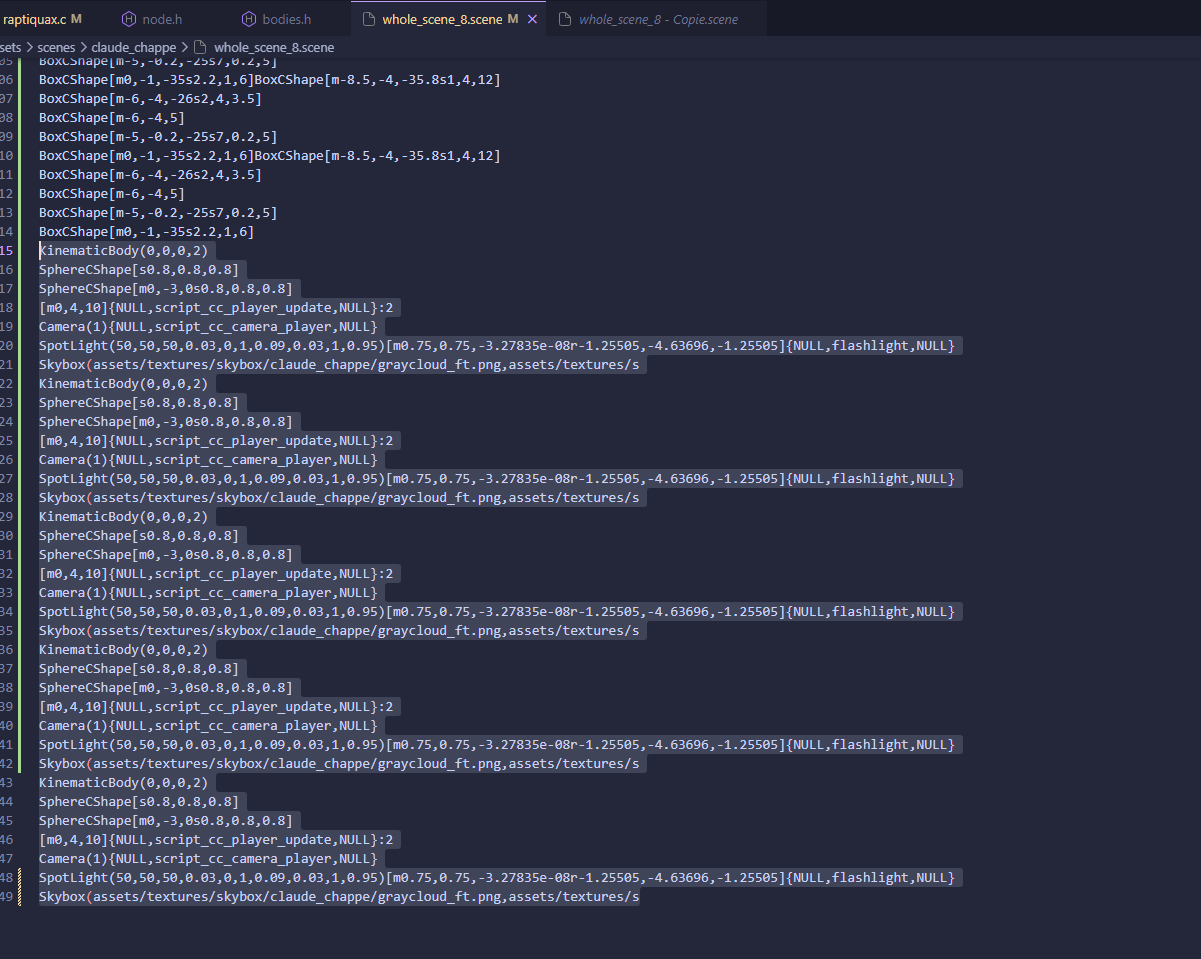
\includegraphics[width=0.5\textwidth]{images/gdb_fix.png}
    \caption{Correction du bug grâce à GDB}
    \label{fig:fix}
\end{figure}
\end{multicols}

\subsection{Code d'une classe générique}
\lstinputlisting[style=class_c,caption={Template de classe dans RaptiquaX},label=lst:class_template]{pages/developpement/class_templace.class.c}
\subsection{Rendu différé}
\label{sec:deferred_rendering}
Exemple de rendu différé :
\begin{figure}[h]
    \begin{subfigure}{0.5\textwidth}
        \centering
        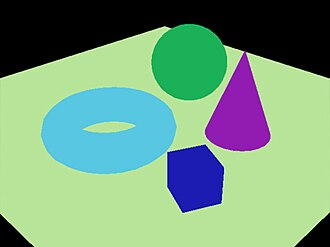
\includegraphics[width=0.8\textwidth]{images/Deferred_rendering_pass_col.jpg}
        \caption{G-Buffer de couleur}
        \label{fig:drendering_pass_col}
    \end{subfigure}
    \begin{subfigure}{0.5\textwidth}
        \centering
        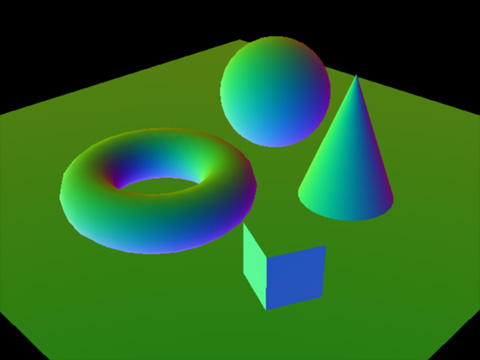
\includegraphics[width=0.8\textwidth]{images/Deferred_rendering_pass_nor.jpg}
        \caption{G-Buffer de normal}
        \label{fig:drendering_pass_normal}
    \end{subfigure}
    \begin{subfigure}{0.5\textwidth}
        \centering
        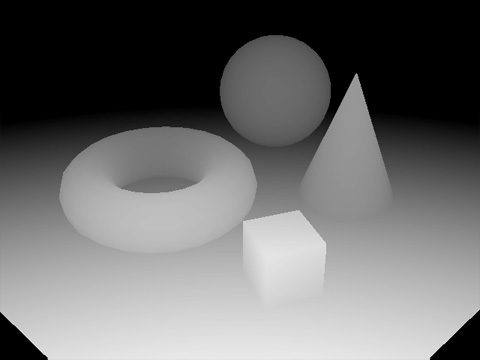
\includegraphics[width=0.8\textwidth]{images/Deferred_rendering_pass_dep.jpg}
        \caption{Z-Buffer}
        \label{fig:drendering_pass_depth}
    \end{subfigure}
    \begin{subfigure}{0.5\textwidth}
        \centering
        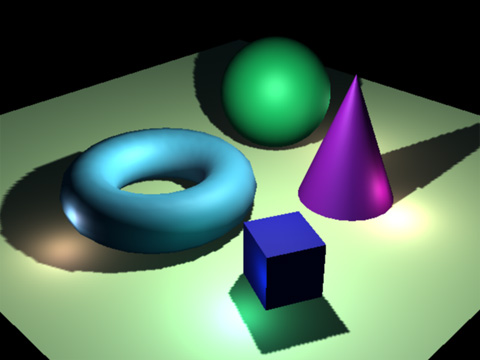
\includegraphics[width=0.8\textwidth]{images/Deferred_rendering_pass_res.jpg}
        \caption{Résultat final}
        \label{fig:drendering_result}
    \end{subfigure}
    \caption{Rendu différé d'une scène de volumes simples}
    \label{fig:defferred_rendering}
\end{figure}

\emph{Ici les Buffers ont été séparés pour montrer les différentes étapes du rendu différé.}

Le rendu différé s'appuie sur un G-Buffer qui contient les informations de la scène,
comme la couleur, les normaux et la profondeur. Ce G-Buffer est calculé en amont, lors
du rendu de la scène. C'est ensuite lors du rendu de la lumière et des effets de
post-processing qu'on utilise ce G-Buffer pour éviter de recalculer les informations de
la scène.
\newpage
\subsection{Pipeline graphique}
    \label{sec:graphics_pipeline}
    \begin{figure}[H]
        \begin{subfigure}{0.5\textwidth}
            \centering
            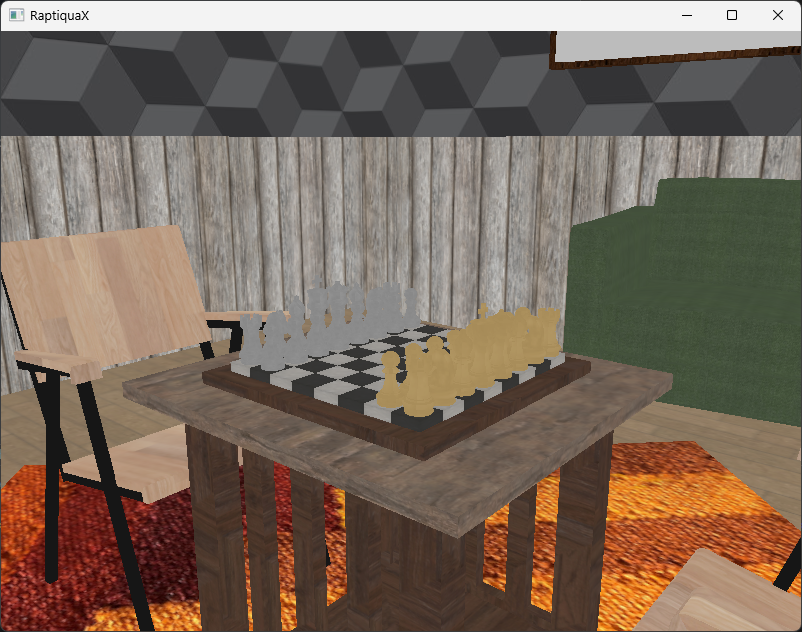
\includegraphics[width=0.8\textwidth]{images/raptiquax_rendering_gbuffer_albedo.png}
            \caption{G-Buffer de couleur}
            \label{fig:graphics_pipeline_gbuffer_albedo}
        \end{subfigure}
        \begin{subfigure}{0.5\textwidth}
            \centering
            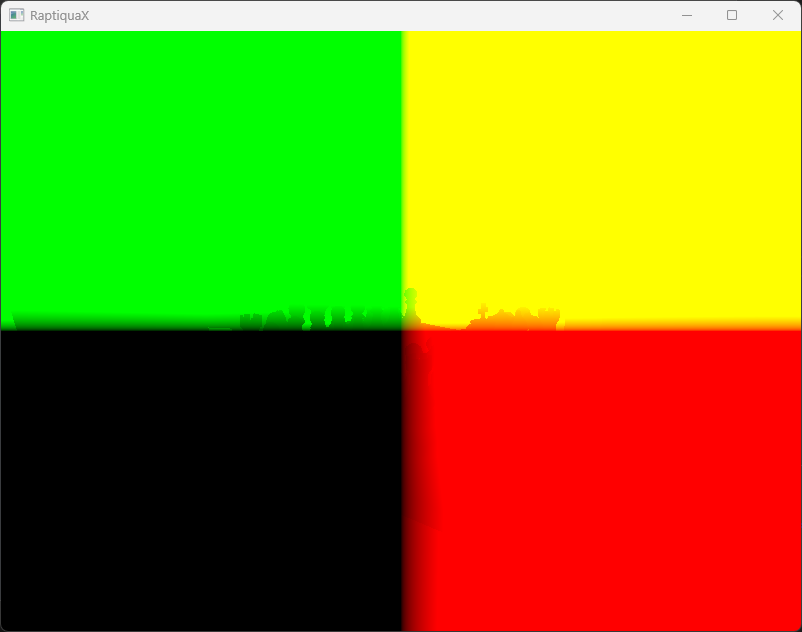
\includegraphics[width=0.8\textwidth]{images/raptiquax_rendering_gbuffer_position.png}
            \caption{G-Buffer de position}
            \label{fig:graphics_pipeline_gbuffer_position}
        \end{subfigure}
        \begin{subfigure}{0.5\textwidth}
            \centering
            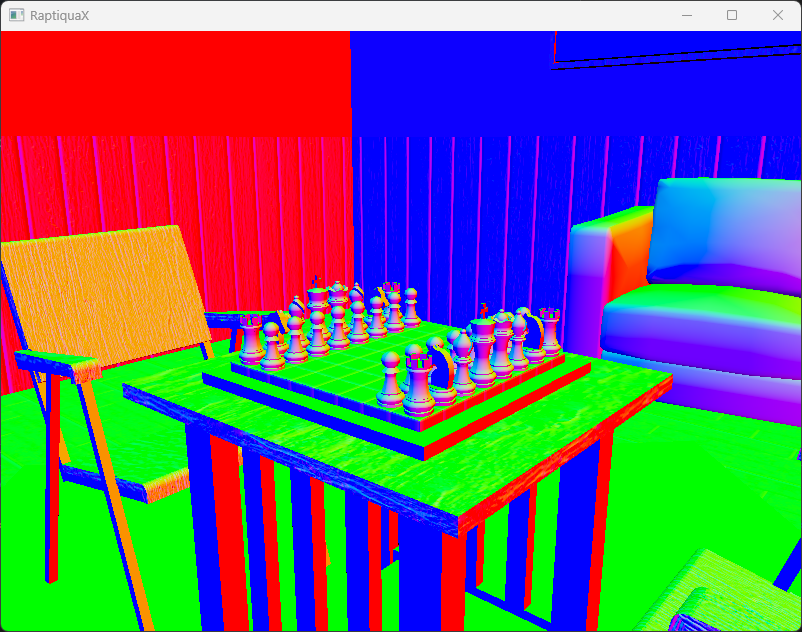
\includegraphics[width=0.8\textwidth]{images/raptiquax_rendering_gbuffer_normal.png}
            \caption{G-Buffer de normal}
            \label{fig:graphics_pipeline_gbuffer_normal}
        \end{subfigure}
        \begin{subfigure}{0.5\textwidth}
            \centering
            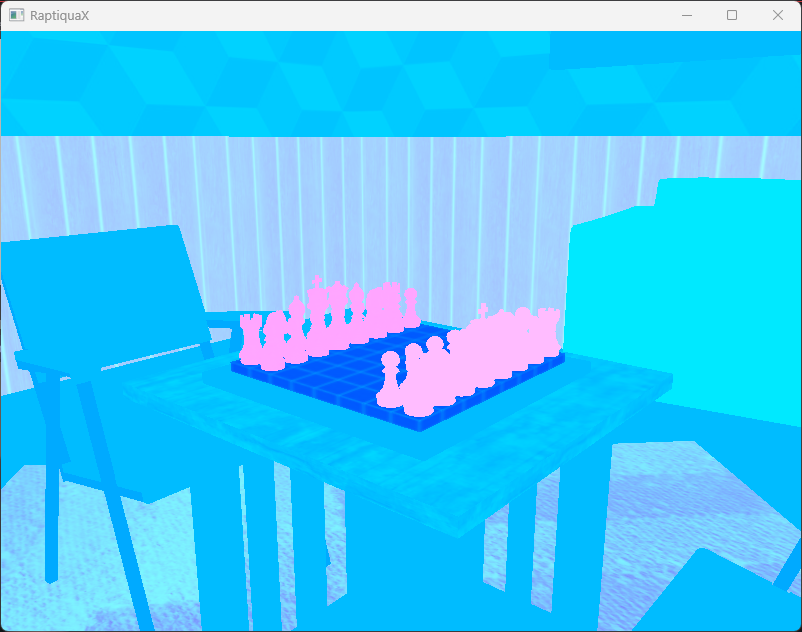
\includegraphics[width=0.8\textwidth]{images/raptiquax_rendering_gbuffer_extra.png}
            \caption{G-Buffer de métallicité et de rugosité}
            \label{fig:graphics_pipeline_gbuffer_color}
        \end{subfigure}
        \caption{G-Buffer de la scène}
        \label{fig:graphics_pipeline_gbuffer}
    \end{figure}
    \begin{figure}[H] 
        \begin{subfigure}{0.3\textwidth}
            \centering
            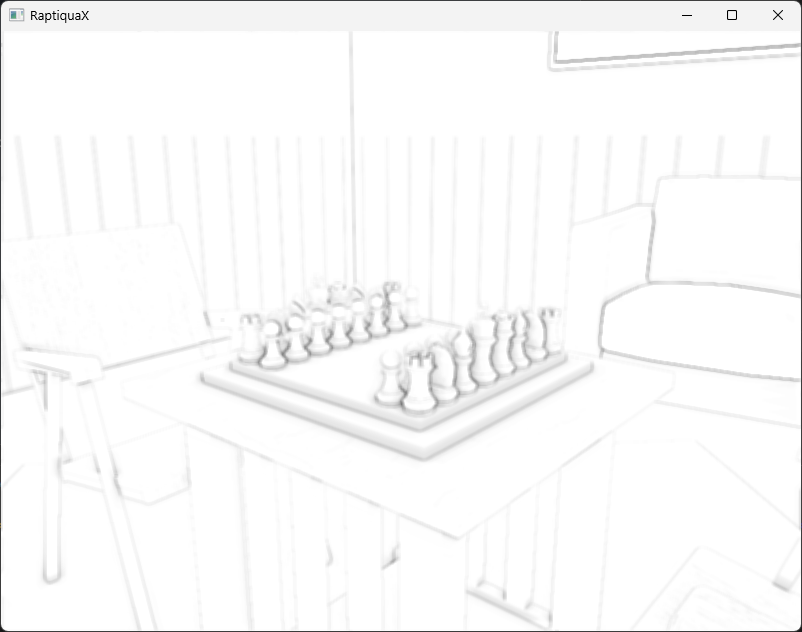
\includegraphics[width=0.8\textwidth]{images/raptiquax_rendering_ssao.png}
            \caption{Calque de l'occlusion ambiante}
            \label{fig:graphics_pipeline_gbuffer_ssao}
        \end{subfigure}
        \begin{subfigure}{0.3\textwidth}
            \centering
            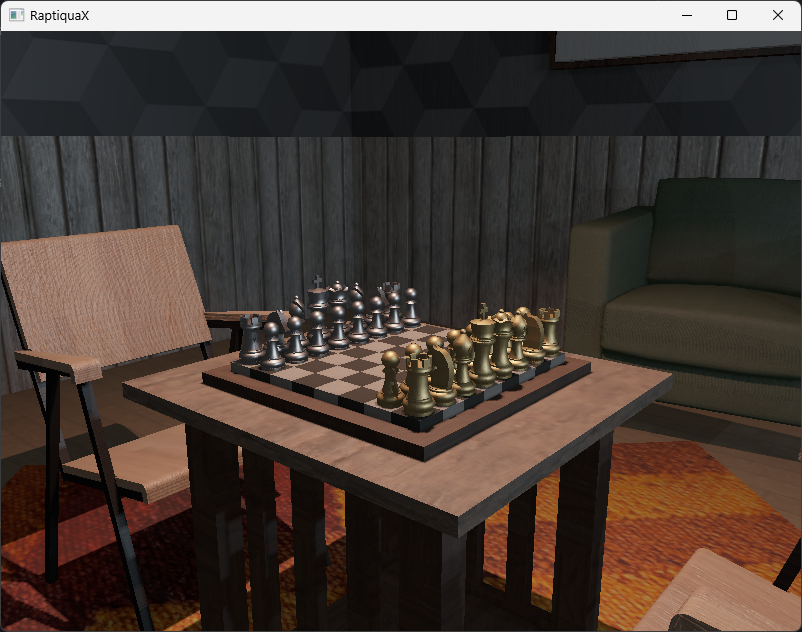
\includegraphics[width=0.8\textwidth]{images/raptiquax_rendering_lightings.png}
            \caption{Calque de la lumière et des ombres}
            \label{fig:graphics_pipeline_gbuffer_light}
        \end{subfigure}
        \begin{subfigure}{0.3\textwidth}
            \centering
            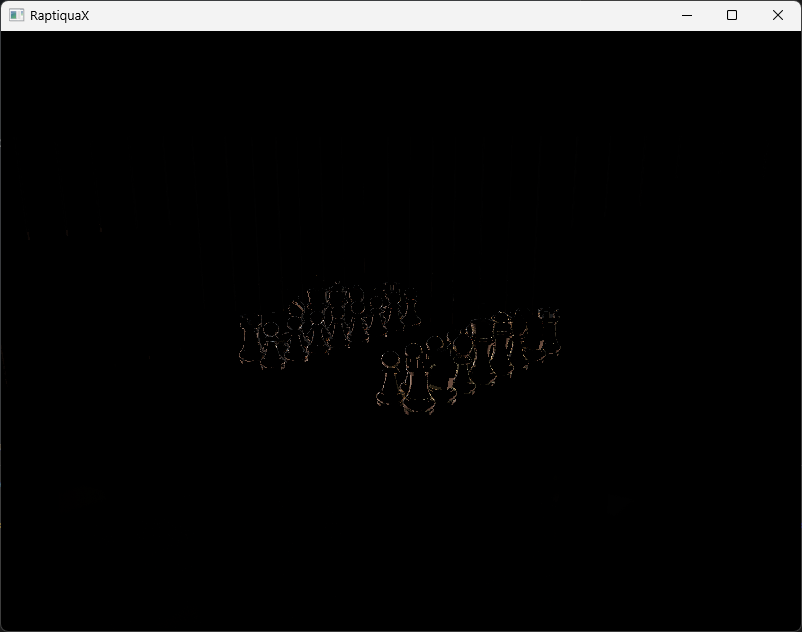
\includegraphics[width=0.8\textwidth]{images/raptiquax_rendering_ssr.png}
            \caption{Calque des réflexion et reflets}
            \label{fig:graphics_pipeline_gbuffer_ssr}
        \end{subfigure}
        \begin{subfigure}{0.3\textwidth}
            \centering
            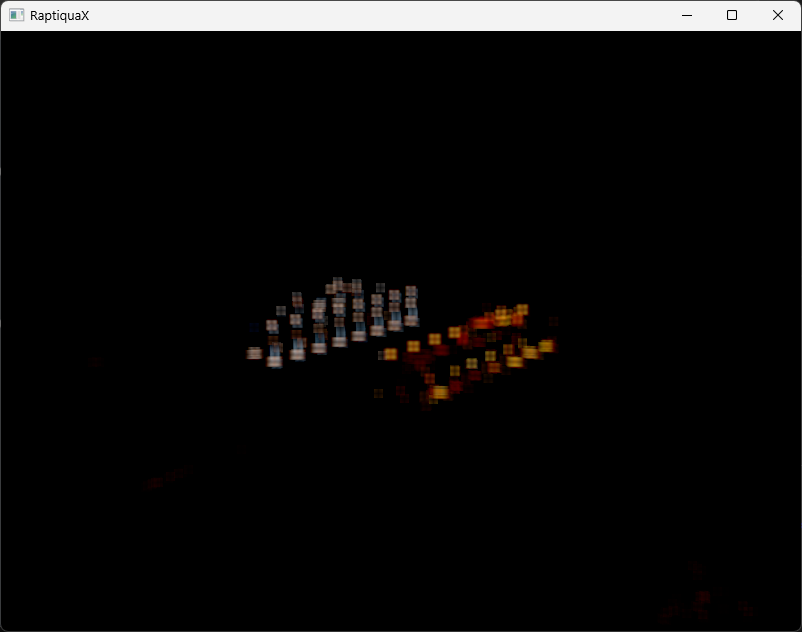
\includegraphics[width=0.8\textwidth]{images/raptiquax_rendering_bloom.png}
            \caption{Calque de l'éblouissement}
            \label{fig:graphics_pipeline_gbuffer_bloom}
        \end{subfigure}
        \begin{subfigure}{0.3\textwidth}
            \centering
            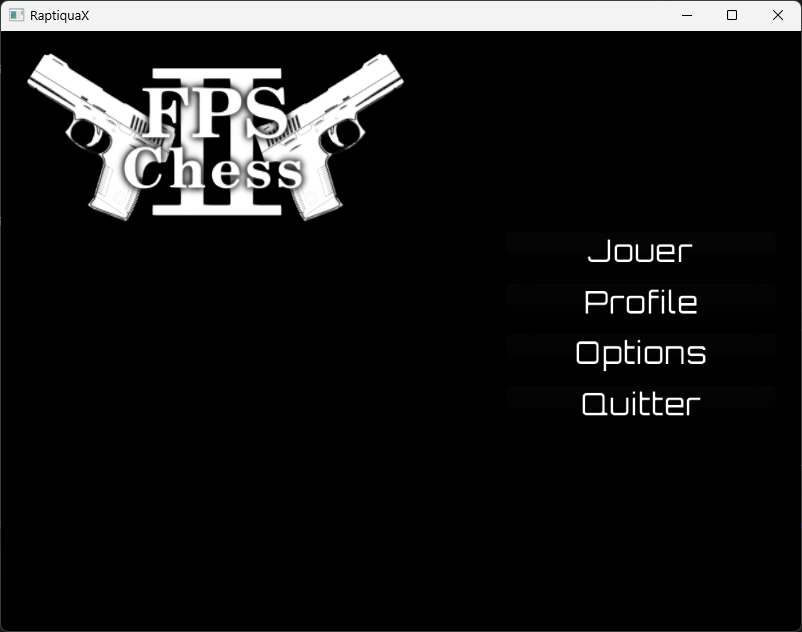
\includegraphics[width=0.8\textwidth]{images/raptiquax_rendering_gui.png}
            \caption{Calque de l'interface utilisateur}
            \label{fig:graphics_pipeline_gbuffer_gui}
        \end{subfigure}
        \caption{Calques de la scène}
        \label{fig:graphics_pipeline_post_processing}
    \end{figure}
    \begin{figure}[H]
        \centering
        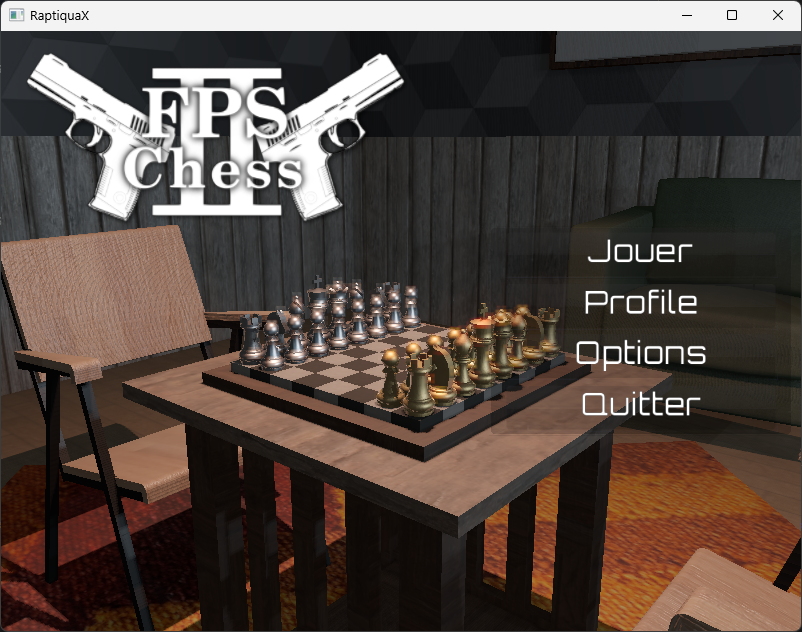
\includegraphics[width=0.5\textwidth]{images/raptiquax_rendering_result.png}
        \caption{Résultat de la pipeline graphique}
        \label{fig:graphics_pipeline_result}
    \end{figure}
\subsection{Musique}
\begin{figure}[H]
    \centering
    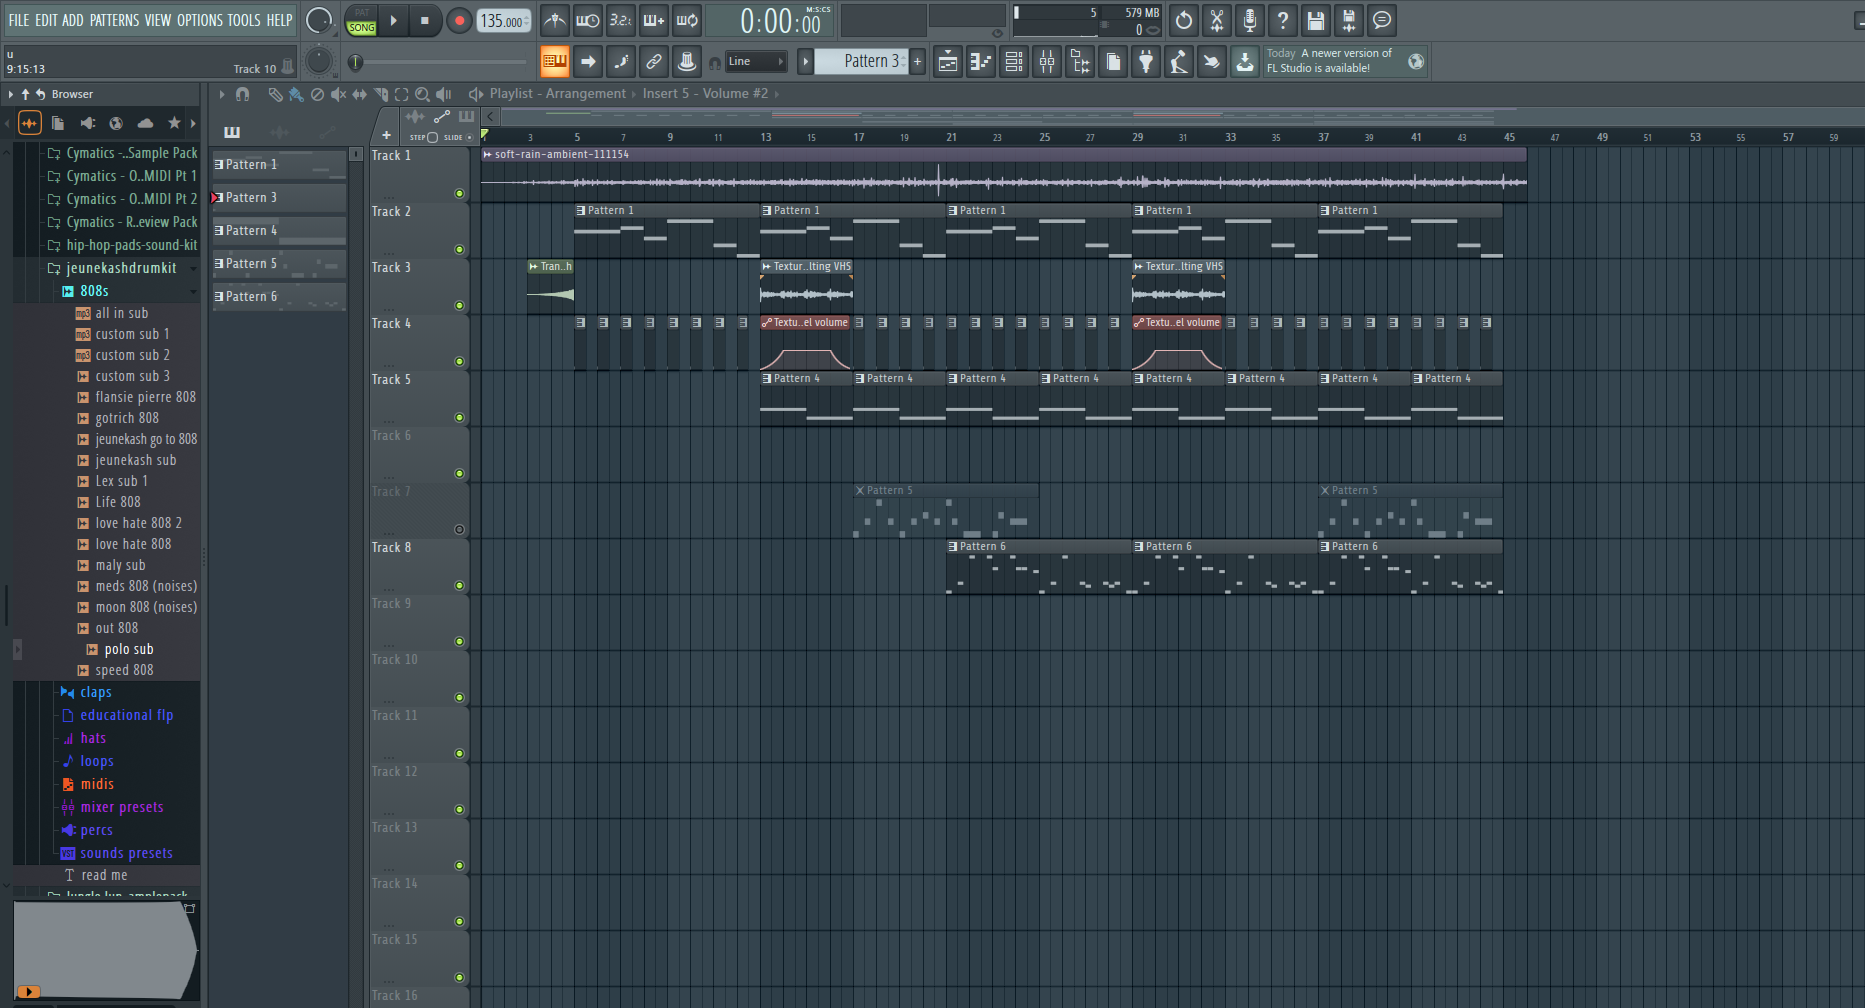
\includegraphics[width=1\linewidth]{images/flstudio.png}
    \caption{fl studio}
    \label{fig:flstudio.png}
\end{figure}

\newpage


\subsection{Équations de la physique}
    \label{sec:physics_equations}
    \paragraph{Norme de la collision}
    La norme de la collision entre les deux corps est donnée par un vecteur
    normal à la surface de collision. Si les corps ont une normale de
    collision définie, cette norme est utilisée dans les calculs suivants.

    \nomenclature{$\mathbf{n}$}{Vecteur normal à la surface de collision}
    \nomenclature{$\mathbf{\lambda}_A$}{Normale de l'objet $A$}
    \nomenclature{$\mathbf{\lambda}_B$}{Normale de l'objet $B$}

    \begin{equation}
    \mathbf{n} = \mathbf{\lambda}_A \cdot \mathbf{\lambda}_B
    \end{equation}

    \paragraph{Vitesse relative}
    La vitesse relative des deux objets rigides \( A \) et \( B \) est calculée
    comme la différence entre leurs vitesses respectives :

    \nomenclature{$\mathbf{v}_{\text{relative}}$}{Vitesse relative entre deux objets}
    \nomenclature{$\mathbf{v}_A$}{Vitesse de l'objet $A$}
    \nomenclature{$\mathbf{v}_B$}{Vitesse de l'objet $B$}

    \begin{equation}
    \mathbf{v}_{\text{relative}} = \mathbf{v}_B - \mathbf{v}_A
    \end{equation}

    \paragraph{Vitesse relative selon la direction normale}
    \nomenclature{$v_{\text{normal}}$}{Vitesse relative projetée sur la normale de collision}

    \begin{equation}
    v_{\text{normal}} = \mathbf{v}_{\text{relative}} \cdot \mathbf{n}
    \end{equation}

    \paragraph{Coefficient de restitution (élasticité de la collision)}
    \nomenclature{$e$}{Coefficient de restitution}

    \begin{equation}
    e = 0.02
    \end{equation}

    \paragraph{Calcul de l'impulsion}
    \nomenclature{$I_{scalaire}$}{Quantité scalaire représentant l'impulsion échangée}
    \nomenclature{$m_A$}{Masse de l'objet $A$}
    \nomenclature{$m_B$}{Masse de l'objet $B$}

    \begin{equation}
    I_{scalaire} = \frac{(1 + e) \cdot v_{\text{normal}}}{m_A^{-1} + m_B^{-1}}
    \end{equation}

    \paragraph{Calcul du vecteur d'impulsion}
    \nomenclature{$\mathbf{I}$}{Vecteur d'impulsion appliqué pendant la collision}

    \begin{equation}
    \mathbf{I} = I_{scalaire} \cdot \mathbf{n}
    \end{equation}

    \paragraph{Application de l'impulsion et du couple}
    \nomenclature{$\mathbf{r}_A$}{Vecteur du centre de masse de $A$ au point d’impact}
    \nomenclature{$\mathbf{r}_B$}{Vecteur du centre de masse de $B$ au point d’impact}
    \nomenclature{$\mathbf{C}_A$}{Centre de masse de $A$}
    \nomenclature{$\mathbf{C}_B$}{Centre de masse de $B$}
    \nomenclature{$\mathbf{P}_{\text{impact}}$}{Point d’impact}

    \begin{equation}
    \mathbf{r}_A = \mathbf{P}_{\text{impact}} - \mathbf{C}_A
    \end{equation}
    \begin{equation}
    \mathbf{r}_B = \mathbf{P}_{\text{impact}} - \mathbf{C}_B
    \end{equation}
    \begin{equation}
    \text{Couple sur A} = \mathbf{r}_A \times \mathbf{I}
    \end{equation}
    \begin{equation}
    \text{Couple sur B} = \mathbf{r}_B \times \mathbf{I}
    \end{equation}

    \paragraph{Application de l'impulsion}
    \nomenclature{$\mathbf{v}_A'$}{Nouvelle vitesse de l’objet $A$}
    \nomenclature{$\mathbf{v}_B'$}{Nouvelle vitesse de l’objet $B$}

    \begin{equation}
    \mathbf{v}_A' = \mathbf{v}_A + \mathbf{I} \cdot m_A^{-1}
    \end{equation}
    \begin{equation}
    \mathbf{v}_B' = \mathbf{v}_B - \mathbf{I} \cdot m_B^{-1}
    \end{equation}

    \paragraph{Correction de la pénétration}
    \nomenclature{$\delta$}{Profondeur de pénétration}
    \nomenclature{$\mathbf{C}$}{Correction appliquée pour compenser la pénétration}
    \nomenclature{$\mathbf{P}_A$}{Position initiale de l'objet $A$}
    \nomenclature{$\mathbf{P}_B$}{Position initiale de l'objet $B$}
    \nomenclature{$\mathbf{P}_A'$}{Nouvelle position de l'objet $A$}
    \nomenclature{$\mathbf{P}_B'$}{Nouvelle position de l'objet $B$}

    \[
    \mathbf{C} = \delta \cdot \mathbf{n}
    \]
    \begin{equation}
    \mathbf{P}_A' = \mathbf{P}_A - \mathbf{C}
    \end{equation}
    \begin{equation}
    \mathbf{P}_B' = \mathbf{P}_B + \mathbf{C}
    \end{equation}

    \paragraph{Calcul du couple et de l'inertie}
    \nomenclature{$\mathbf{I}_{\text{locale}}$}{Matrice d’inertie locale}
    \nomenclature{$w$}{Largeur de l'objet}
    \nomenclature{$h$}{Hauteur de l'objet}
    \nomenclature{$d$}{Profondeur de l'objet}

    \begin{equation}
    \mathbf{I}_{\text{locale}} = \frac{m}{12} \begin{bmatrix} h^2 + d^2 & 0 & 0 \\ 0 & w^2 + d^2 & 0 \\ 0 & 0 & w^2 + h^2 \end{bmatrix}
    \end{equation}

    \paragraph{Accélération angulaire}
    \nomenclature{$\mathbf{\alpha}$}{Accélération angulaire}
    \nomenclature{$\mathbf{T}$}{Couple appliqué}
    \nomenclature{$\mathbf{I}^{-1}$}{Inverse de la matrice d’inertie}

    \begin{equation}
    \mathbf{\alpha} = \mathbf{I}^{-1} \cdot \mathbf{T}
    \end{equation}

\subsection{Tableau des différents n\oe{}uds de la scène}
    \renewcommand{\arraystretch}{1.2}
    \setlength{\tabcolsep}{10pt}

    \begin{longtable}{>{\bfseries}p{0.25\linewidth} p{0.7\linewidth}}
        \toprule
        \textbf{Nœud} & \textbf{Description} \\
        \midrule
        Node & Classe de base pour tous les objets de la scène \\
        Camera & Représente un point de vue pour le rendu \\
        BoxCShape & Forme de collision en boîte \\
        CapsuleCShape & Forme de collision en capsule \\
        CShape & Classe de base des formes de collision \\
        MeshCShape & Forme de collision basée sur un maillage \\
        PlaneCShape & Plan infini utilisé pour les collisions \\
        RayCShape & Détecteur de collision basé sur un rayon \\
        SphereCShape & Forme de collision sphérique \\
        Button & Élément d'interface cliquable \\
        CheckBox & Case à cocher \\
        ControlFrame & Conteneur pour organiser l'interface \\
        Frame & Conteneur de base pour l'interface \\
        ImageFrame & Cadre affichant une image \\
        InputArea & Champ de saisie de texte \\
        Label & Étiquette de texte \\
        SelectList & Liste déroulante ou défilable \\
        Slider & Curseur pour sélectionner une valeur \\
        DirectionalLight & Source lumineuse directionnelle (\textit{ex : soleil}) \\
        Light & Classe de base pour les sources de lumière \\
        PointLight & Lumière omnidirectionnelle ponctuelle \\
        SpotLight & Source lumineuse en forme de cône \\
        Mesh & Maillage basique sans texture \\
        Model & Modèle 3D complet et texturé \\
        Area & Zone invisible déclenchant des événements \\
        Body & Classe de base pour les corps physiques \\
        KinematicBody & Corps physique contrôlé manuellement \\
        RigidBody & Objet physique entièrement simulé \\
        StaticBody & Corps physique immobile \\
        PhysicalNode & Base pour les nœuds liés à la physique \\
        RenderTarget & Sous scène rendu dans une texture \\
        Skybox & Cube d'environnement représentant le ciel \\
        TexturedMesh & Maillage avec textures appliquées \\
        \bottomrule
        \caption{Liste des n\oe{}uds de la scène}
        \label{tab:raptiquax_nodes}
    \end{longtable}

\subsection{Tableau des commandes Socket du mini-jeu \og FPS Chess \fg{}}
    \begin{table}[H]
        \centering
        \scriptsize
        \renewcommand{\arraystretch}{1.1}
        \begin{tabular}{|l|p{2.5cm}|p{4.5cm}|}
            \hline
            \textbf{Commande} & \textbf{Arguments} & \textbf{Description} \\
            \hline
            PONG & Aucun & Répond au ping du serveur. \\
            LOGIN & Nom d'utilisateur & Authentifie l'utilisateur et enregistre son nom. \\
            CREATE\_PARTY & Nom de la partie & Crée une nouvelle partie avec un nom donné. \\
            LIST\_PARTY & Aucun & Liste les parties existantes. \\
            EXIT\_PARTY & Aucun & Quitte la partie actuelle. \\
            JOIN\_PARTY & ID de la partie & Rejoint une partie donnée (par ID). \\
            RENAME\_PARTY & Nouveau nom & Renomme la partie actuelle. \\
            PARTY\_SET\_DATA & Clé=Valeur & Définit une valeur clé dans les données de la partie. \\
            PARTY\_GET\_DATA & Clé & Récupère une valeur clé des données de la partie. \\
            PARTY\_GET\_SELF\_INDEX & Aucun & Récupère l'index du joueur dans la partie. \\
            EXIT & Aucun & Déconnecte le client du serveur. \\
            G\_MSG & Message & Envoie un message global aux autres clients connectés. \\
            MSG & Message & Envoie un message à tous les joueurs de la partie ou globalement si hors partie. \\
            \hline
        \end{tabular}
        \caption{Requêtes gérées par le serveur SocketIO du moteur RaptiquaX}
        \label{tab:raptiquax_requests}
    \end{table}